%%%%%%%%%%%%%%%%%%%%% chapter.tex %%%%%%%%%%%%%%%%%%%%%%%%%%%%%%%%%
%
% sample chapter
%
% Use this file as a template for your own input.
%
%%%%%%%%%%%%%%%%%%%%%%%% Springer-Verlag %%%%%%%%%%%%%%%%%%%%%%%%%%
%\motto{Use the template \emph{chapter.tex} to style the various elements of your chapter content.}

% Chapter Template

\chapter{Smoothed Particle Hydrodynamics} % Main chapter title

\label{Chapter 5} % Change X to a consecutive number; for referencing this chapter elsewhere, use \ref{ChapterX}

%----------------------------------------------------------------------------------------
%	SECTION 1
%----------------------------------------------------------------------------------------

\section{Mesh-free methods}
In this chapter the meshfree methods are introduced and explained on the example of the Smoothed Particle
Hydrodynamics method. For further reading Liu2003 is recommended.

\subsection{Why use mesh free methods?}

As described in Chapter 3 the scientific and engineering community have used mesh-based methods for
very long as they have cleary matured over the years. Still
Capability to work from
micro to macro scale applications.

The benefits of mesh-free methods versus classical mesh-based methods can be outlined as:
\begin{itemize}
\item Mesh-free methods can easily handle strong deformations that would lead to
remeshing in a FEM simulation. This is due to the absence of a topological mesh which in course
of a deformation simulation would lead to problems in connectivity. ShafonLi 15
\item The mesh-free discretization with particals can provide a better representation of a varying
geometric shape.
\end{itemize}

In this report we will focus on the Smoothed Particle Hydrodynamics method as one of the earliest
and vastly used mesh-free methods.

\subsection{History of SPH}

The idea of SPH was at first formulated in the year 1977. Its origins do not lie in CFD but in the attempt to model and solve astrophysical problems in a new way. Initially Gingold and Monoghan Gingold1977 invented and named this approach at the Institute of Astronomy in Cambridge. Their primary intention was to find a approach that would be less computational intensive than FDM to solve various evolution processes (e.g. a star forming from interstellar matter). In their article they state how limited the use of FDM
is for their often asymmetrical/distorted problems, since in order to be be computed accurately they needed a excessive amount of grid points (resp. high spatial discretization). They proposed a new way of discretization that was based on a Lagrangian description and used a fixed amount of randomly distributed particles. To model physical scalar and vector fields and to retrieve those values during computation they used statistical methods (Monte Carlo integral determination) along with a \emph{kernel function}. Their approach will be described in more detail in the following sections.  
Inspired by the colleagues at Cambridge, Lucy Lucy1977 used this numerical approach to test succesfully the feasability of the fission hypothesis for protostars, which is a gas dynamical problem of rotating fluids in space. In contrast to CFD, these problems like the formation of galaxies or solar systems are of macroscopic scale.
Today SPH and its further developments are widely adapted in astronomy, CFD and even VFX. 


\subsection{Applications of SPH}
Because of several numerical advantages of SPH it is today not only used in astrophysics but also in a wide
range of simulations for fluid dynamics like underwater explosions (e.g. Liu et al. ) and even fluid creation
for visual effects in feature film (see Chapter 4...) One of this visual effects applications will be explained
in more detail with the SPH software "Realflow" and NAIAD. For further reading on the applications of CFD in computer graphics please refer to Bridson2008 and for new Hybrid Methods that have the advantages of Meshbased and Meshfree methods pg. 195 Jackl2006 provides a simple introduction. 


\begin{figure}[htp]
\centering
\begin{tabular}{cccc}
	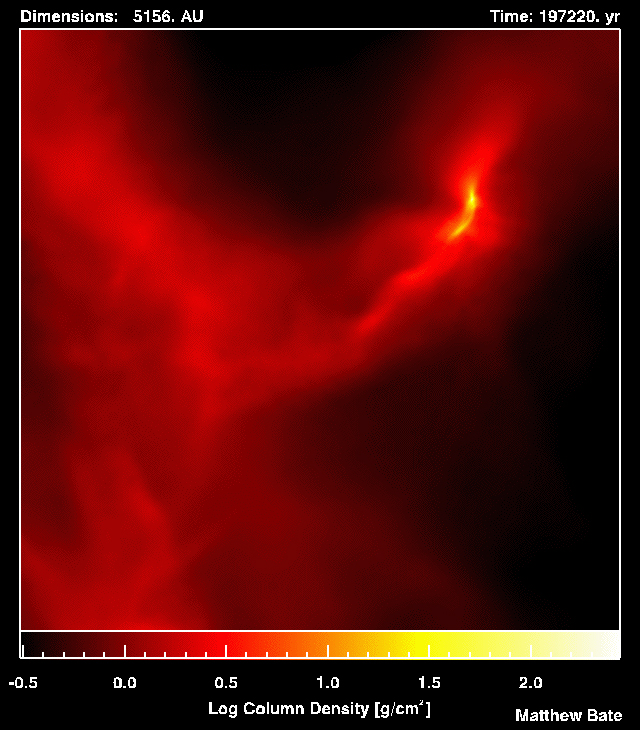
\includegraphics[width=0.2\textwidth]{../figures/sph_bates_starcluster_00.jpg} 
 &  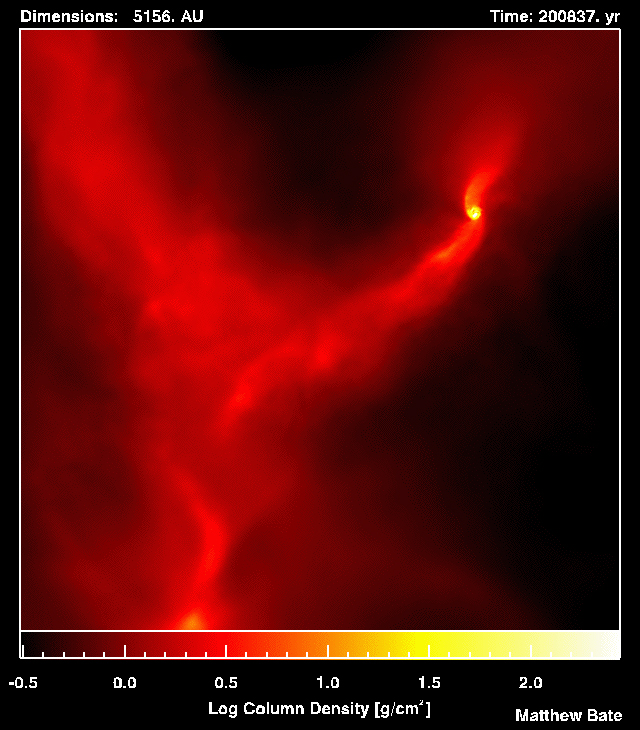
\includegraphics[width=0.2\textwidth]{../figures/sph_bates_starcluster_01.jpg}
 &  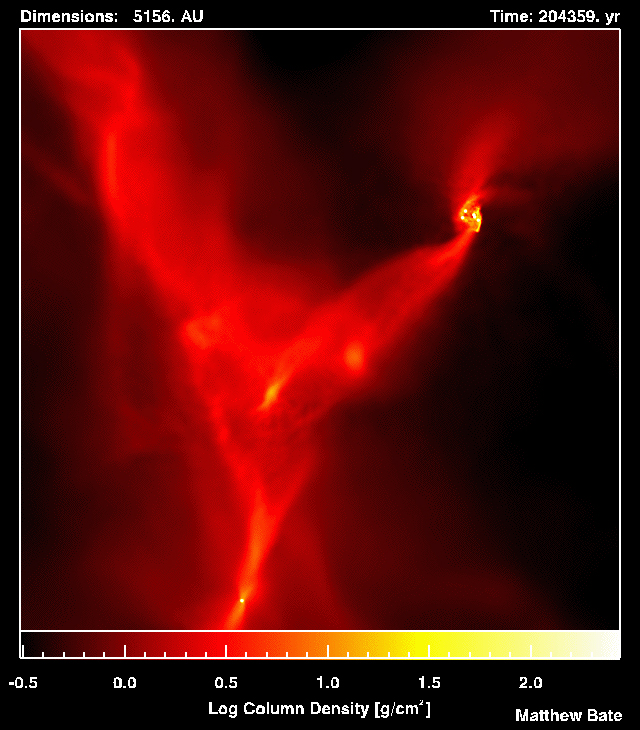
\includegraphics[width=0.2\textwidth]{../figures/sph_bates_starcluster_02.jpg}
 &  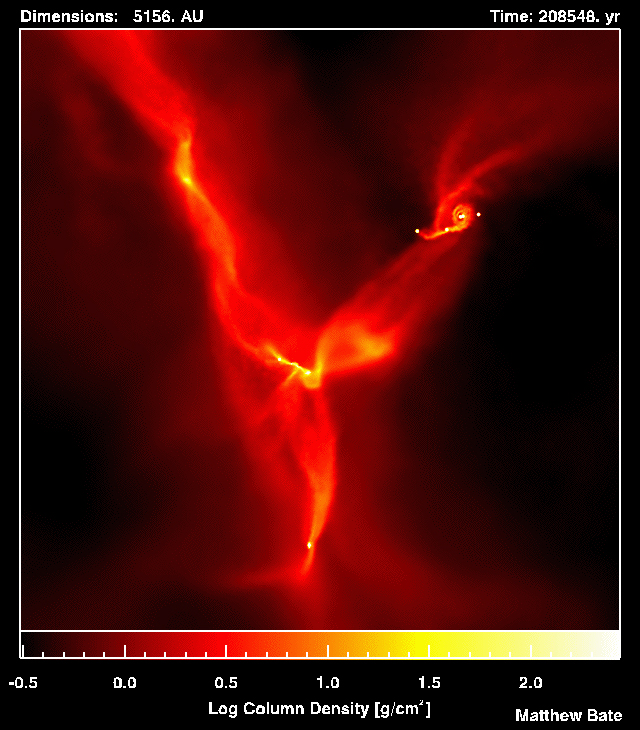
\includegraphics[width=0.2\textwidth]{../figures/sph_bates_starcluster_03.jpg}  
 \\
	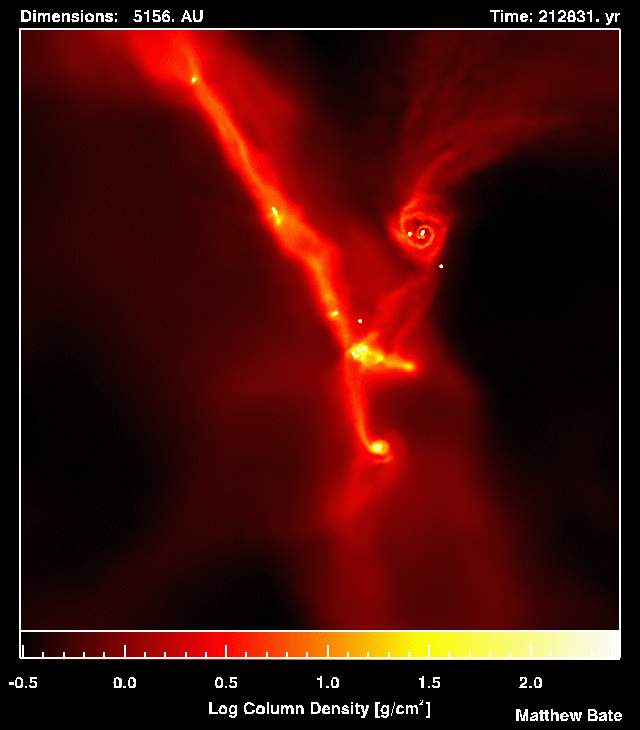
\includegraphics[width=0.2\textwidth]{../figures/sph_bates_starcluster_04.jpg} 
 &  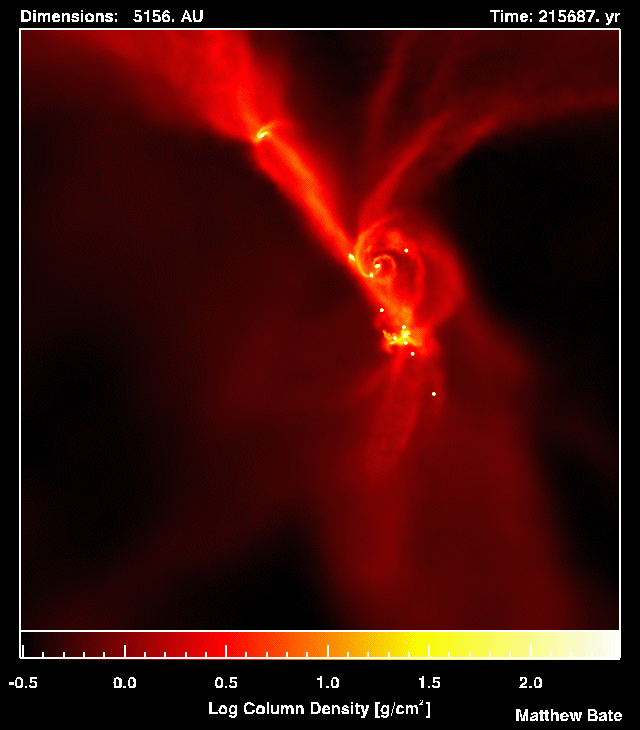
\includegraphics[width=0.2\textwidth]{../figures/sph_bates_starcluster_05.jpg} 
 &  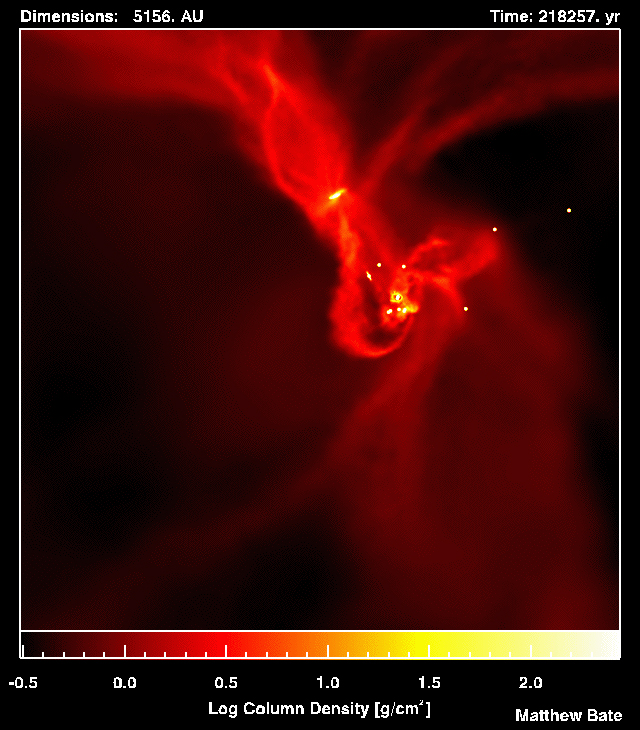
\includegraphics[width=0.2\textwidth]{../figures/sph_bates_starcluster_06.jpg}
 &  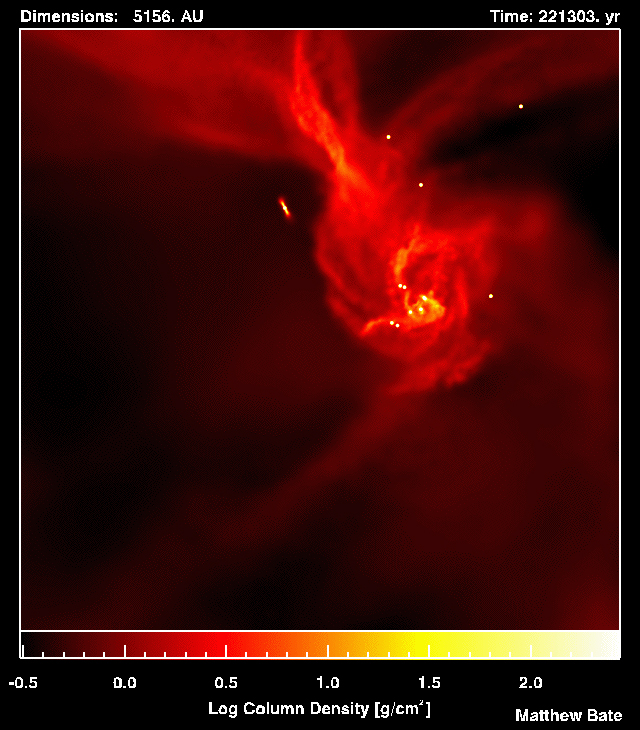
\includegraphics[width=0.2\textwidth]{../figures/sph_bates_starcluster_07.jpg} 
 \\
	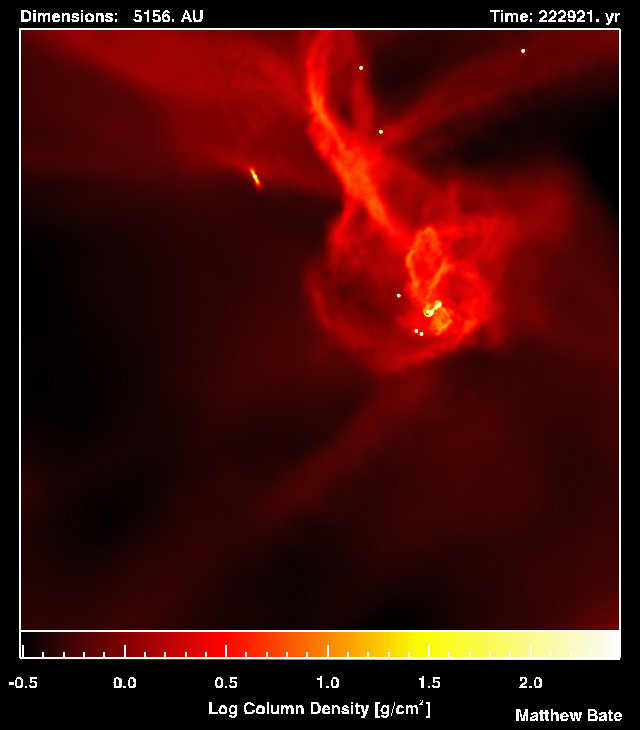
\includegraphics[width=0.2\textwidth]{../figures/sph_bates_starcluster_08.jpg} 
&   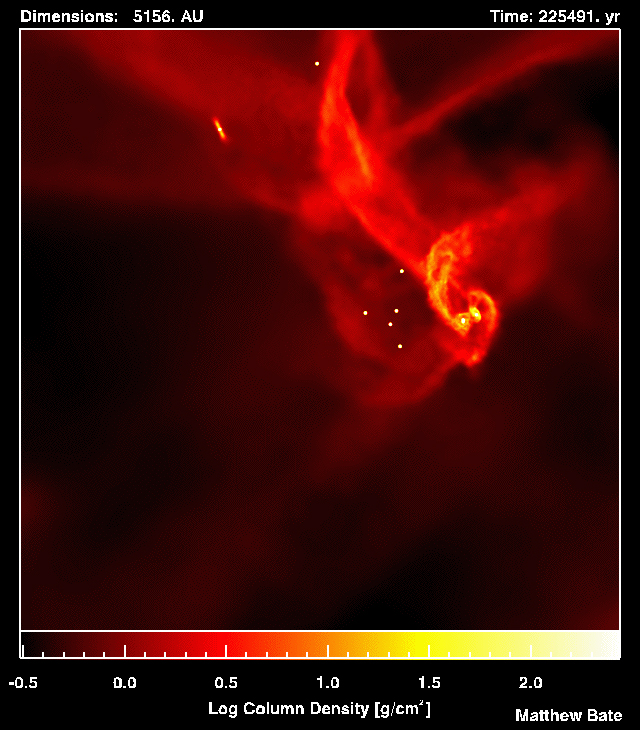
\includegraphics[width=0.2\textwidth]{../figures/sph_bates_starcluster_09.jpg}  
&   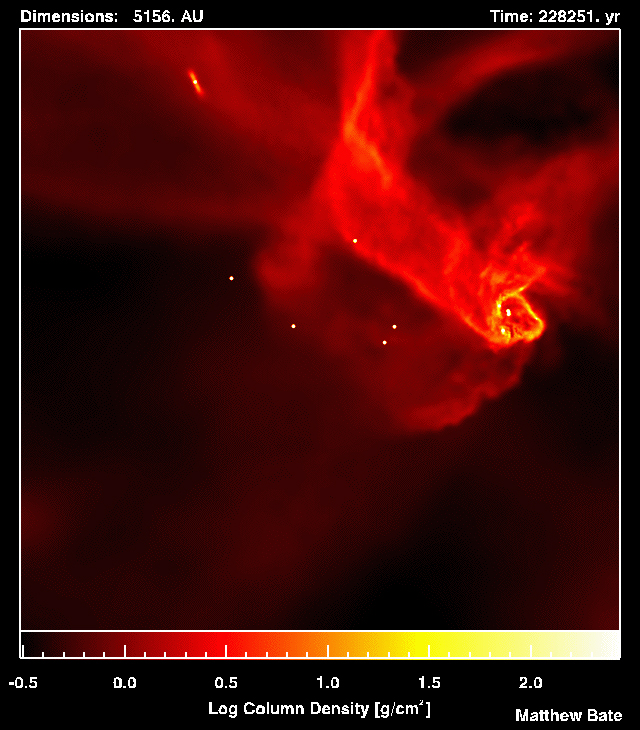
\includegraphics[width=0.2\textwidth]{../figures/sph_bates_starcluster_10.jpg}
&   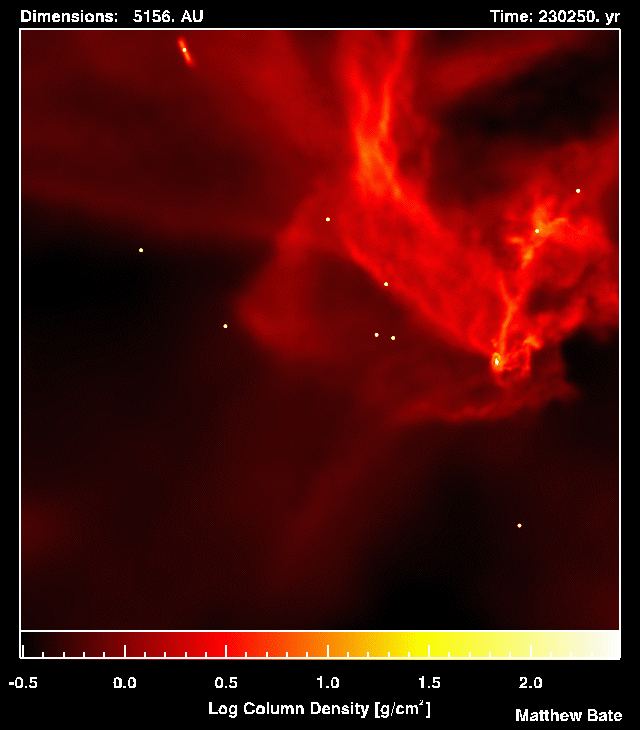
\includegraphics[width=0.2\textwidth]{../figures/sph_bates_starcluster_11.jpg} 
\\
	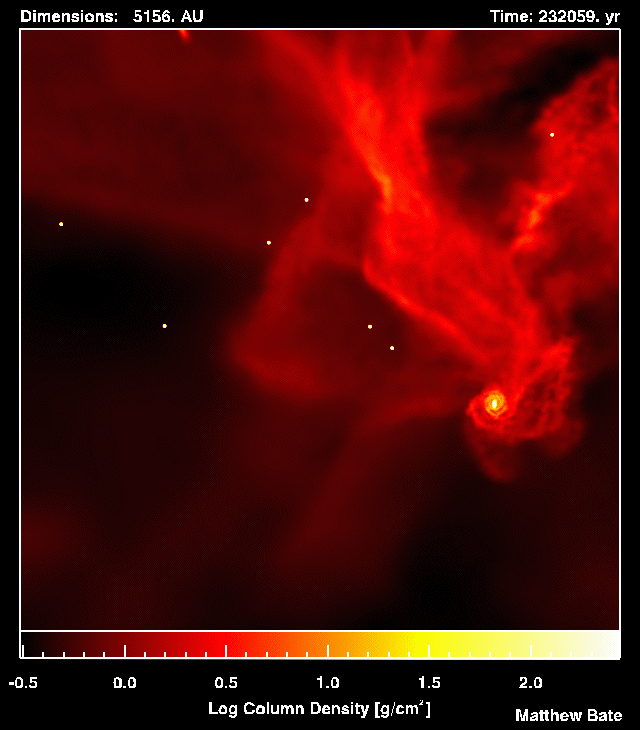
\includegraphics[width=0.2\textwidth]{../figures/sph_bates_starcluster_12.jpg} 
&   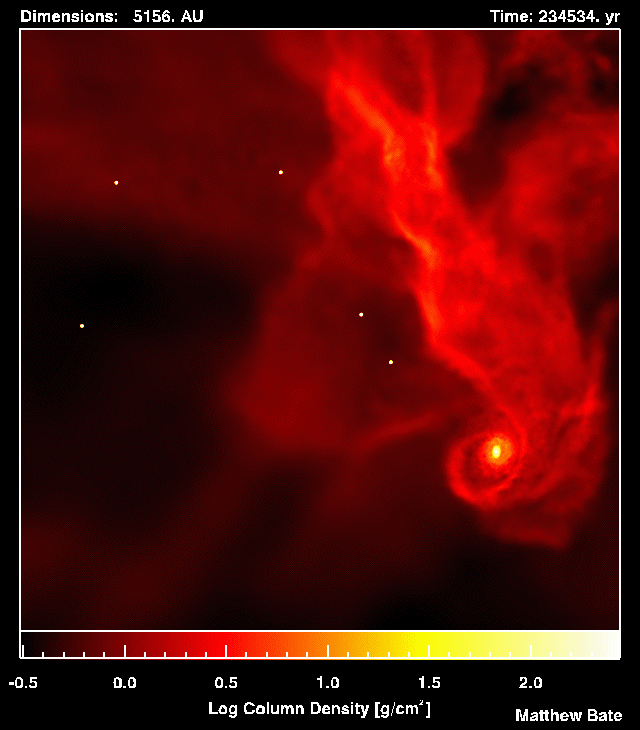
\includegraphics[width=0.2\textwidth]{../figures/sph_bates_starcluster_13.jpg}  
&   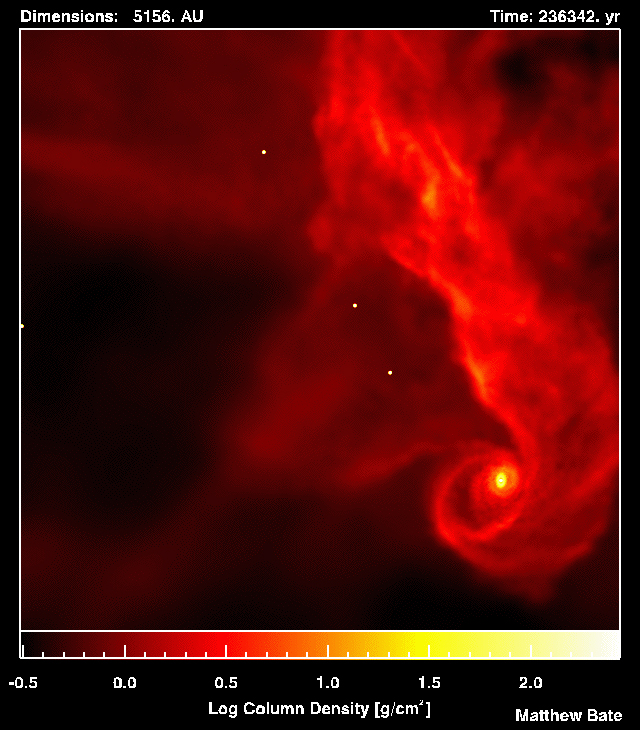
\includegraphics[width=0.2\textwidth]{../figures/sph_bates_starcluster_14.jpg}
&   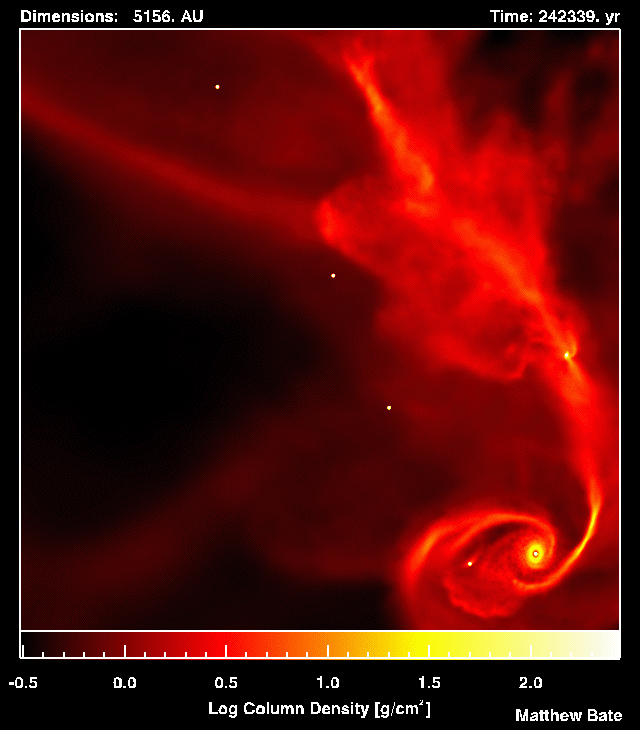
\includegraphics[width=0.2\textwidth]{../figures/sph_bates_starcluster_15.jpg}
\\

\end{tabular}
\caption{Image sequence of the Formation of Stars and Brown Dwarfs in a Star Cluster}
\label{fig:SPHStarCluster}
\end{figure}

\subsection{Basic idea of SPH}
SPH is a so called meshfree particle method (MPM) and replaces the meshbased discretization with a initial distribution of particles over the problem domain. 

\section{Mathematical foundation}

In order to discretize a domain with particles, the mathematical foundations differ greatly from Meshbased methods. Similar to FVM a integral representation of fluid variables is needed. For a continuous function $f(x)$ that has the mathematical preconditions to be represented in a integral form, it can be written in integral form as follows:

\begin{equation} \label{eq:func_intg_dirac}
f(x) = \int_{\Omega} \biggl [ f(a) \delta(x-a) \biggr ] d a \ \ \ (x, a) \in \Omega
\end{equation}

With the Dirac delta function being:

% \begin{equation}
% \label{eq:dirac_delta_fu}
% \delta(x-a)= 
% \begin{cases}
% 1, &\mbox{if } x = a \\ 
% 0, & \mbox{if } x \neq a
% \end{cases}
% \end{equation}


Where $ \Omega $ represents the problem domain with the vectors $ x  a $ in it. Because of the Dirac delta function \ref{eq:dirac_delta_fu} the integral formulation becomes zero at all vectors except the exact vector x. The form \ref{eq:func_intg_dirac} is of great importance to SPH methods. It allows the Dirac delta function $\delta$ (which produces a exact equality)  to be replaced by a \emph{kernel function} K which leads to the approximation:

\begin{equation} \label{eq:func_intg_kernel}
f(x) \approx \int_{\Omega} \biggl [ f(a) K(x-a) \biggr ] d a \ \ \ (x, a) \in \Omega
\end{equation}

In the equations of fluid dynamics, often the divergence operator is found. The divergence of a vector function $\nabla \cdot f(x)$ can be similarly
written like the above notation:

\begin{equation} \label{eq:func_intg_kernel_div}
\nabla \cdot f(x) \approx \int_{\Omega} \biggl [ \nabla \cdot f(a) K(x-a) \biggr ] d a \ \ \ (x, a) \in \Omega
\end{equation}
 

In the following section this kernel function is further discussed in brought into a form where it can be discretized.

\subsection{Kernel approximation}
The kernel function K can be rewritten with another parameter $h$, which as we will see is used for a similar limit formulation, as it is found in the equations of Meshbased methods. Furthermore due to a already established conventions in SPH, the bracket operator $ < >$ is used to 
clearly visualize that function $f(x)$ is approximated by the kernel function K:

\begin{equation} \label{eq:func_intg_kernel_h_brk}
< f(x) > = \int_{\Omega} \biggl [ f(a) K(x-a, h) \biggr ] d a \ \ \ (x, a) \in \Omega
\end{equation}

The bracket operator can be also used to rewrite equation \ref{eq:func_intg_kernel_div}:

\begin{equation} \label{eq:func_intg_kernel_h_brk_div}
< \nabla \cdot f(x) > = \int_{\Omega} \biggl [ \nabla \cdot f(a) K(x-a, h) \biggr ] d a \ \ \ (x, a) \in \Omega
\end{equation}

The relation between the Dirac delta function and the kernel function K can be written down with the limit notation by:

\begin{equation} \label{eq:kernel_vs_dirac}
\lim_{h \to 0} K(x-a, h) = \delta(x-a)
\end{equation}

Similar to equation \ref{eq:fdm_con} in FDM, the value of $ h $ is used to approximate a function. In contrast to FDM though, not the function itself that should be discretized is approximated, but the Dirac function. Equation \ref{eq:kernel_vs_dirac} represent the \emph{Delta function condition}, which is one out of three conditions that has to be met my the kernel function K, in order to be used with SPH. For further reading on the \emph{unity condition} and the \emph{compact condition} please refer to pg. 37 Liu2003. From now on we will call $ h $ the kernel \emph{length}. In literature the term \emph{kernel} is often used in exchange with the term \emph{smoothing}, which result in smoothing function K and smoothing length $h$. In this report the term kernel will be used. The problem domain $ \Omega $ is also called \emph{support domain}.\footnote{This is a simplification. Strictly speaking the support domain can also be outside of the problem domain and therefore not equivalent.}  

The equation \ref{eq:func_intg_kernel_h_brk_div} can be rewritten to: 

\begin{equation} \label{eq:func_intg_kernel_h_brk_div}
< \nabla \cdot f(x) > = 
\overbrace{\int_{\Omega} \nabla \cdot \biggl [ f(a) K(x-a, h) \biggr ] d a}^{Divergence\ theorem\ applicable} -
\int_{\Omega} \biggl [ f(a) \cdot \nabla K(x-a, h) \biggr ] d a
\end{equation}

This form allows to apply the divergende theorm, onto the RHS of the equation:

\begin{equation} \label{func_intg_kernel_h_brk_div_theo}
< \nabla \cdot f(x) > = 
\int_{A} \biggl [ f(a) K(x-a, h) \cdot \vec{n}  \biggr ] d A -
\int_{\Omega} \biggl [ f(a) \cdot \nabla K(x-a, h) \biggr ] d a
\end{equation}

For vectors a which are not identical to vector x, and for which the distance between them bypasses the kernel length  $|(x-a)| > h $  the kernel function becomes zero. This leads the integral of the surface A which is located inside the problem domain $\Omega$ to be zero. Therefore the equation simplifies to:

\begin{equation} \label{eq:func_intg_kernel_simple}
< \nabla \cdot f(x) > = 
- \int_{\Omega} \biggl [ f(a) \cdot \nabla K(x-a, h) \biggr ] d a
\end{equation}

Considering the conversion of equation \ref{eq:func_intg_kernel_div} to \ref{eq:func_intg_kernel_simple} with the help of the divergence theorem, something remarkable has happened. The divergence operation on the vector function $f(x)$ has been shifted to be a gradient operation at the kernel function K, leaving the vector function untouched. Therefore the kernel approximation in SPH which was used to represent the field function f in a integral form has the following advantage: When a divergence operation occurs at the field function (which often happens in CFD), the solution can be computed by the values of the function itself and the gradient of the kernel function, without caring about the divergence of the function. This will lead to much simpler and faster solvable equations. Now that the continuous integral forms are written in the kernel approximation form, in the next step the equations \ref{eq:func_intg_kernel_h_brk} and \ref{eq:func_intg_kernel_simple} can be finally discretized using particles.

\subsection{Particle approximation}

In order to discretize the continuous integral form that are represented by the kernel approximations, the SPH method uses particle summations. In the beginning of the process the domain is discretized or better split up into randomly distributed system of particles. These particles carry certain values like mass and density. The problem of correctly distributing the particles is further discussed in the Implementation sections of this report. 
In discretized form the particles represent the overall domain $\Omega$. To compute the physical values at a certain point (or particle) inside the domain, the surrounding particles are considered and a weighted average value is computed. This entire process will be discussed in this Section.

For simplicity and better understanding we first assume a already discretized domain with randomly distributed particles. Figure \ref{fig:sph_par_approx_domain} illustrates the two dimensional distribution of these particles in the domain $\Omega$. The region from which field information should be computed is marked as the red particle $i$. This particle is surrounded by a \emph{support domain} (dotted quadratic line) that defines which particles have influence on the field variable values it inhibits. This support domain is controlled by the kernel function K and its kernel length $h$. In the illustration the support domain is simplified as a two dimensional area, but it can also be a spheric volume with radius $h$ or of any other shape that depends on the kernel length. The magnitude of influence is illustrated by
a bell shaped kernel function, that clearly decreases with increasing distance from the particle $i$. Now to transform the idea of this illustration into the mathematical particle approximation of SPH, we consider the support domain to be a cubic volume $V$  with side length $h$.


\begin{figure}[htb]
\centering
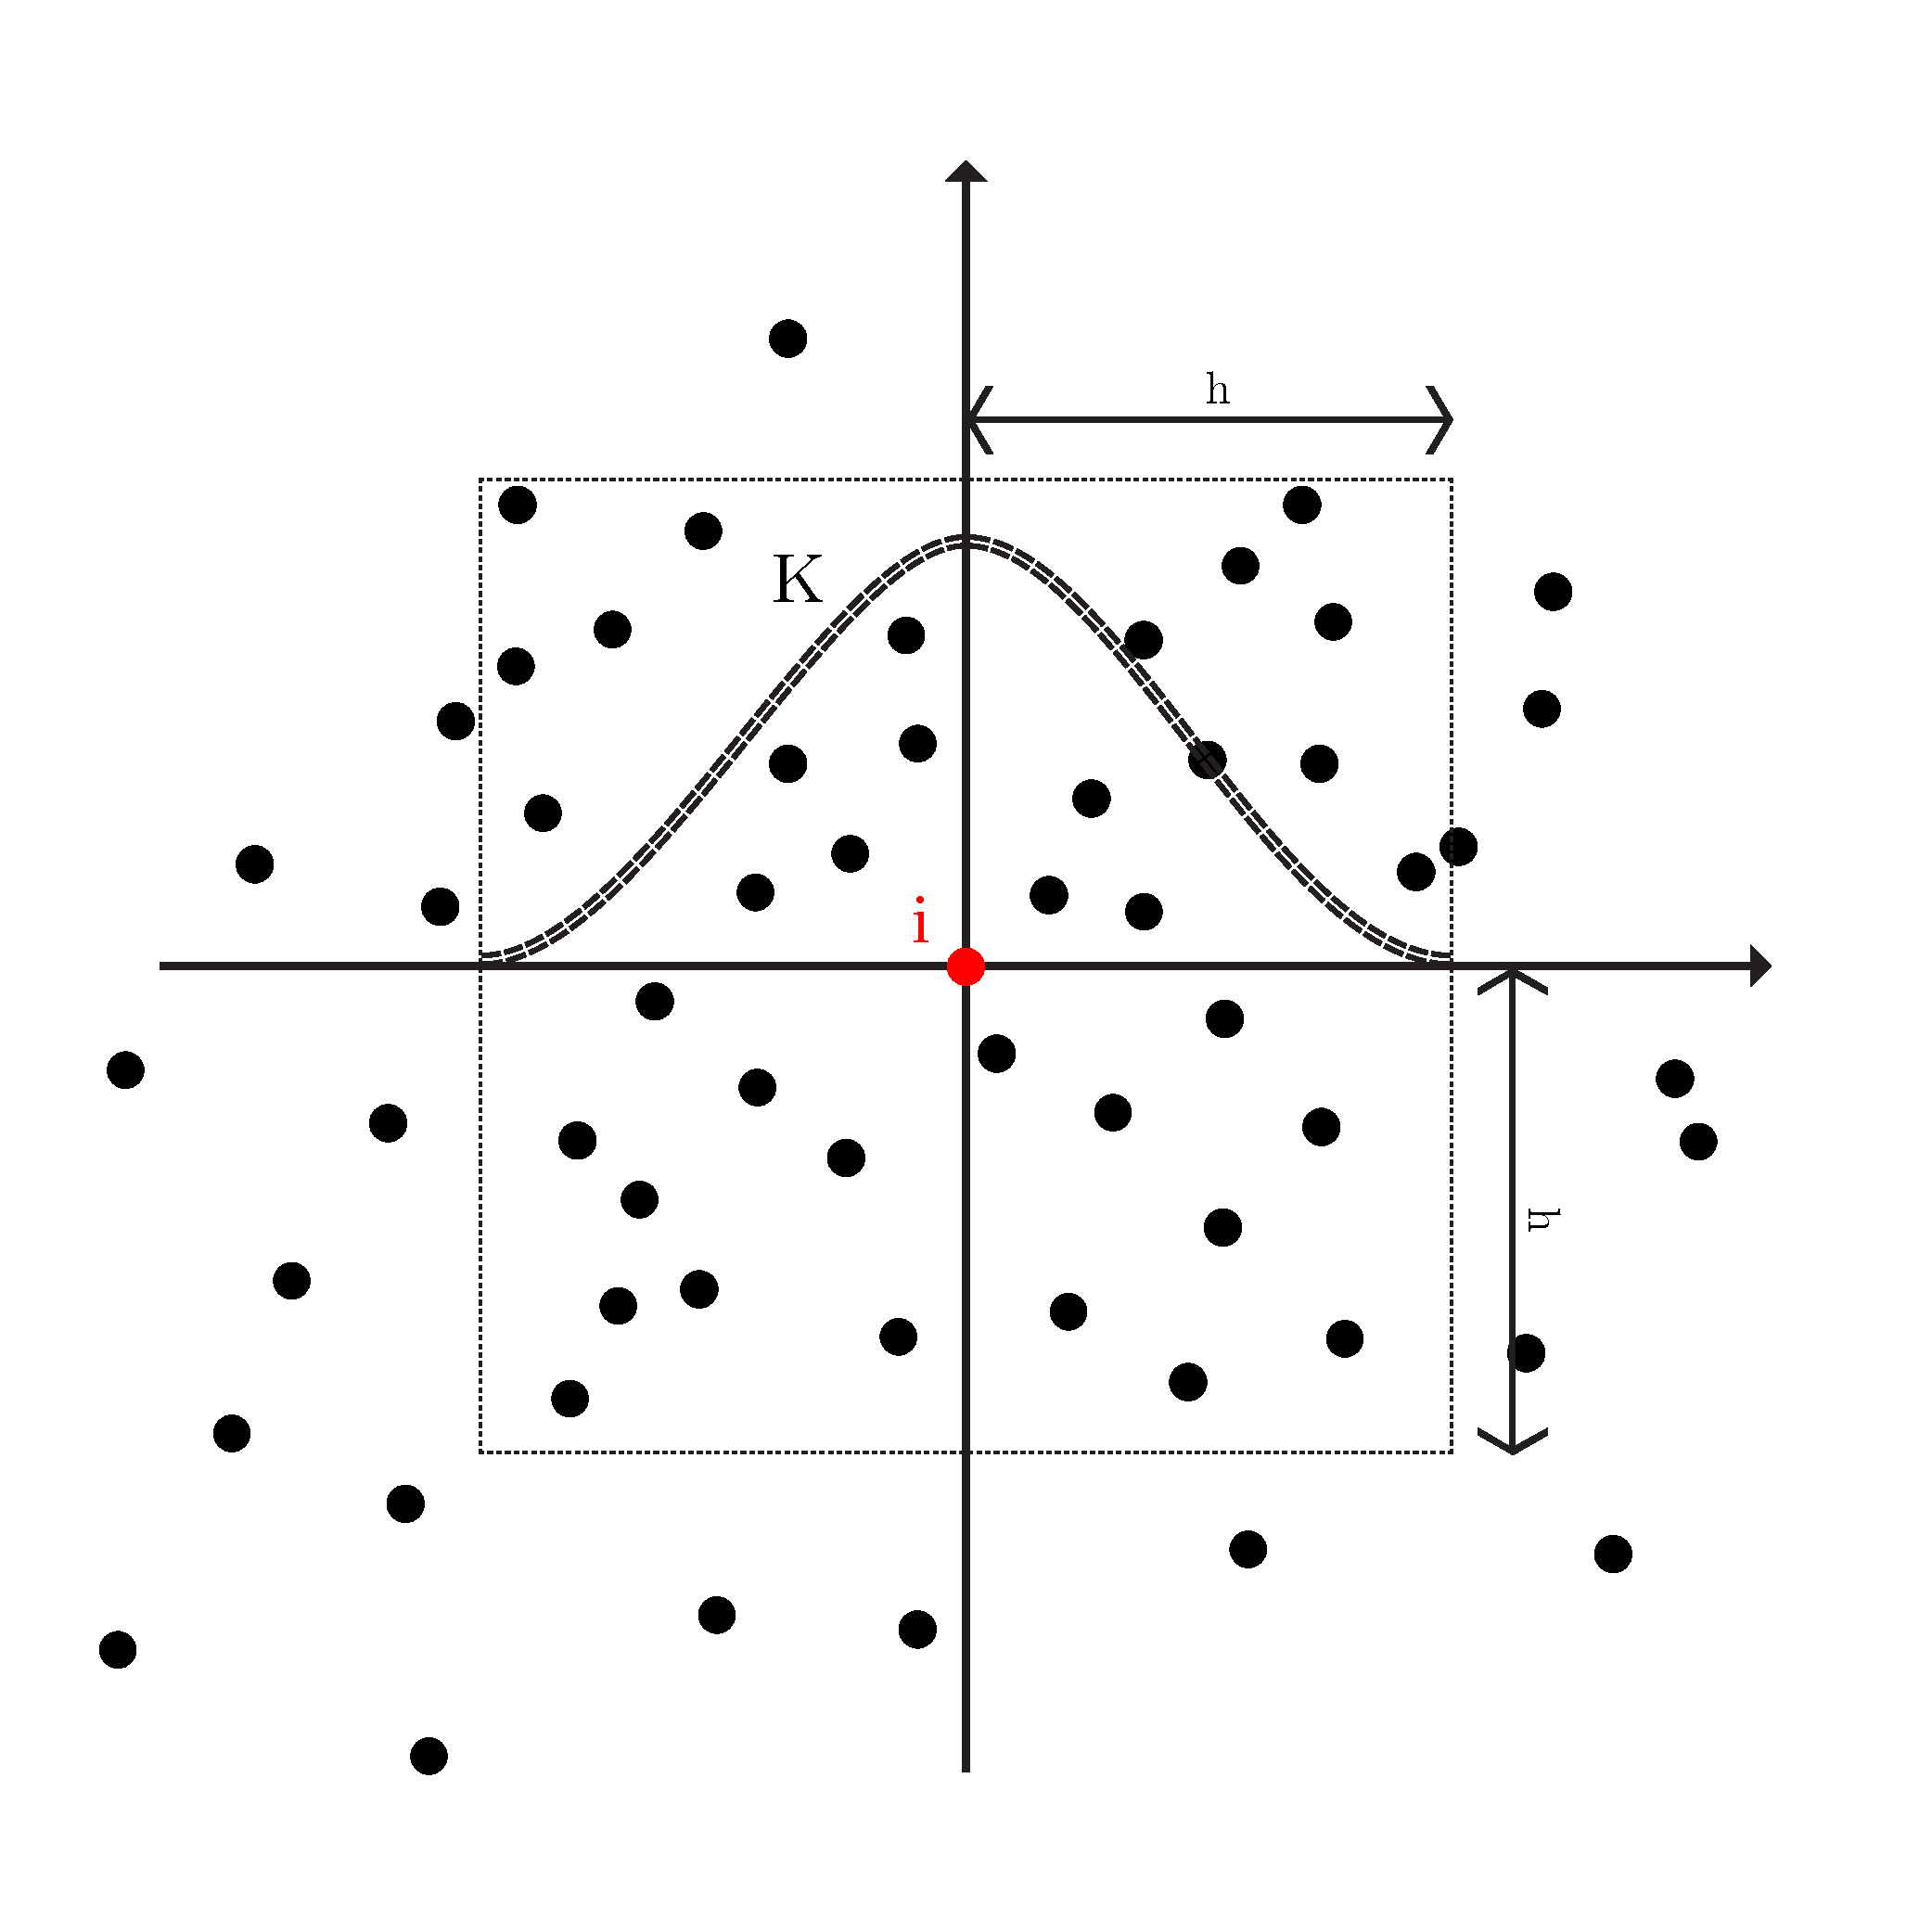
\includegraphics[width=0.8\textwidth]{../figures/sph_particle_domain.pdf}
\caption{Illustration of particle approximation with kernel function K and quadratic support domain}
\label{fig:sph_par_approx_domain}
\end{figure}

The domain $\Omega$ is discretized into a finite amount of $N$ particles. Each particle $j$ is assigned a mass $m_{j}$ and a density $\rho_{j}$, which are equal fractions of the total mass and density of $\Omega$. The mass of particles $m_{j}$ inside the cubic support volume $V_{j}$ can therefore be written as:

\begin{equation} \label{eq:sph_volume_mass}
m_{j} = V_{j}\rho_{j} \ \ \ j \in V_{j}
\end{equation}

Considering the kernel approximation equation \ref{eq:func_intg_kernel_h_brk}, the integral over the continuous domain $\Omega$ can now be rewritten to a discrete summation:

% \begin{equation} 
% \label{eq:kernel_to_part_approx}
% \begin{split}
% < f(x_{i}) > 
% &= \int_{\Omega} \biggl [ f(a) K(x-a, h) \biggr ] d a \\
% &\approx    \sum_{j=1}^{N} \biggl [ f(a_{j}) K(x_{i}-a_{j}, h) V_{j} \biggr ]
% \end{split}
% \end{equation}

In equation \ref{eq:kernel_to_part_approx} the step from kernel approximation to particle approximation has been made. Now the vectors $x_{i}$, $a_{j}$ represent particle positions. Thereby the function is approximated at particle $i$. This equation can be further written with a rearranged equation \ref{eq:sph_volume_mass} in mind to:

% \begin{equation} 
% \label{eq:kernel_to_part_approx_mass_dens}
% \begin{split}
% < f(x_{i}) > 
% &\approx    \sum_{j=1}^{N} \biggl [ f(a_{j}) K(x_{i}-a_{j}, h) V_{j} \biggr ] \\
% &=          \sum_{j=1}^{N} \biggl [ f(a_{j}) K(x_{i}-a_{j}, h) \frac{m_{j}}{\rho_{j}} \biggr ] \\
% &=          \sum_{j=1}^{N} \biggl [ \frac{m_{j}}{\rho_{j}}  f(a_{j}) K(x_{i}-a_{j}, h) \biggr ] 
% \end{split}
% \end{equation}

Note that in equation \ref{eq:kernel_to_part_approx_mass_dens} the only changing input values are the particle properties (e.g. position, mass, density, ...) of the  the particle(s) $i,j$. Furthermore the most significantly varying element in the equation is the kernel function K itself. Most SPH methods can be clearly identified by the kernel function they use to weight the influence of surrounding particles. Therefore the equation can become cleaner by separating the kernel function $K_{i,j}$ 
from the description:

\begin{equation} 
\label{eq:kernel_to_part_clean}
< f(x_{i}) > =
\sum_{j=1}^{N} \frac{m_{j}}{\rho_{j}}  f(a_{j}) \cdot K_{i,j}
\end{equation}

Similar to the kernel approximation in equation \ref{eq:func_intg_kernel_h_brk} the particle approximation can be applied to \ref{eq:func_intg_kernel_simple}, which finally leads to:

\begin{equation} \label{eq:kernel2_to_part_clean}
< \nabla \cdot f(x) > = 
- \sum_{j=1}^{N} \frac{m_{j}}{\rho_{j}}  f(a_{j}) \cdot \nabla K_{i,j}
\end{equation}

In this Section the kernel approximations were discretized to the particle approximations. These two approximations and the step to latter are the mathematical cornerstone of the SPH method. The continuous integrals from the kernel approximations were transformed to summations over a finite amount of particles inside a finite support domain. This particle approximation is done at each time step of the simulation. Note that this simple idea of a averaged summations with particles was done completely without the presence of a mesh. Each particle was associated with at least properties for position, mass and density. As we will see in later Sections, further physical properties can be associated with particles for hydrodynamic problems. How the distribution of particles is done, will be discussed in later Sections. In the following Sections these mathematical framework is used to implement the NSE with SPH. Hereby to consider are algorithms to efficiently determine, which particles are inside the support domain.



\subsection{Lagrangian Navier-Stokes equations}
Because SPH is a pure Lagrangian method, also the NSE need to be formulated in the Lagrangian form. In the previous Chapters mostly the Eulerian forms were used. 

\subsection{SPH vs. FEM}
While both methods in most implementations share a Lagrangian perspective the main difference between the
FEM and particle based methods is indeed the absence of a overall grid in the SPH methods. While FEM is based
on finite elements, they still exist within a grid.

For further reading please refer to Li2004 and Liu2003.

\subsection{Benefits of Meshfree methods over Meshbased methods}
The most problems of the Meshbased methods result not from the numerical capabilities of their methods, but from the simple presence of a mesh itself. 

item Be@tter to model physcal behaviour that has strong distortion
item Mesh dependend problems like re³meshing are avo§ided
item No tie-consuming (re-)genera§tion of meshes for a problem 

%-----------------------------------
%	SUBSECTION 2
%-----------------------------------
\section{Implementation}

\subsection{Nearest neighbour particles}

\subsection{Issues of computer implementation}
%RAM...

\subsection{Par Coding}


Fitc


\section{Implementation of Navier-Stokes equations}


\section{Particle consistency problem}

